\documentclass[oneside,11pt]{article}

\usepackage{blindtext, fancyhdr, newfloat, caption, graphicx}
\usepackage{authblk}
\usepackage[margin=1in]{geometry}
\usepackage{listings}
\usepackage{fancyvrb}
\usepackage{xcolor,colortbl}

\lstset{
        language=C++,
        basicstyle=\small\bfseries,
        %numberstyle=,
        stepnumber=1,
        numbersep=5pt,
        showspaces=false,
        showstringspaces=false,
        showtabs=false,
        frame=none,
        tabsize=2,
        %captionpos=b,
        breaklines=true,
        breakatwhitespace=false,
        escapeinside={\%*}{*)}
}

\lstset{morekeywords={pragma, omp, target, device, data, end, declare
    teams,num\_teams,thread\_limit,map,to,map,from,tofrom,
    parallel},emphstyle={\bfseries}}

% Example environment.
\DeclareFloatingEnvironment[placement={!ht},name=Example]{example}



\pagestyle{fancy}

\title{\textbf{OpenMP offload infrastructure in LLVM}}

\author{
  Samuel Antao (IBM),
  Carlo Bertolli (IBM),
  Andrey Bokhanko (Intel),
  Alexandre Eichenberger (IBM),
  Hal Finkel (Argonne National Laboratory),
  Sergey Ostanevich (Intel),
  Eric Stotzer (Texas Instruments),
  Guansong Zhang (AMD)
}


\begin{document}\thispagestyle{empty}
\maketitle

% Definitions used in the document, e.g. directives, code snippets.

% OpenMP directives, clauses, and modifiers used in the document.
\newcommand{\ompdirectiveclause}[1]{\textbf{\textit{#1}}}

\newcommand{\dtarget}{\ompdirectiveclause{target}}
\newcommand{\dtargetdata}{\ompdirectiveclause{target data}}
\newcommand{\dtargetupdate}{\ompdirectiveclause{target update}}

\newcommand{\ddeclaretarget}{\ompdirectiveclause{declare target}}
\newcommand{\denddeclaretargeta}{\ompdirectiveclause{end declare target}}

\newcommand{\cdevice}{\ompdirectiveclause{device}}
\newcommand{\cmap}{\ompdirectiveclause{map}}
\newcommand{\cto}{\ompdirectiveclause{to}}
\newcommand{\cfrom}{\ompdirectiveclause{from}}

\newcommand{\mto}{\ompdirectiveclause{to}}
\newcommand{\mfrom}{\ompdirectiveclause{from}}
\newcommand{\mtofrom}{\ompdirectiveclause{tofrom}}

% Format of commands.
\newcommand{\command}[1]{\textit{\texttt{#1}}}

% Format of code.
\newcommand{\code}[1]{{\lstinline!#1!}}

% Format of libomptarget.so
\newcommand{\libomptarget}[1]{\texttt{libomptarget.so}}




\section{OpenMP 4.5 offloading overview}\label{sc:OpenMP offloading overview}

The OpenMP 4.5 specification defines offloading directives that can be used to take advantage of accelerators or devices, in OpenMP terminology (see the OpenMP 4.5 specification at www.openmp.org).
\begin{itemize}
  \item \textbf{Device}: an implementation-defined logical execution unit. The execution model is host-centric such that a host device offloads code and data to target devices.

  \item \textbf{Target} regions are structured code blocks that execute on a target device. This is conditional on the run-time availability of a device, the ability of the compiler to generate device code, and other factors. 

  \item \textbf{Target declarations} are used to specify mapping of global variables to a device and create device specific versions of functions that can be called from target regions.

  \item \textbf{Device data environments} contain the variables that are currently present on the target device.

  \item \textbf{A mapped variable} is a variable in a (host) data environment with a corresponding variable in a device data environment.

\end{itemize}

The \dtarget{} directive creates both a device data environment and a target region. It may have associated clauses to specify further details, like the exact device to use if more than one is present in the system (\cdevice{} clause) or whether the data should be moved to/from the device or only allocated in the device memory (\cmap{} clause). The \ddeclaretarget{} directive declares that enclosed global variables and functions should have corresponding device versions.

Example~\ref{ex:OffloadingExample} illustrates how offloading can be expressed using the available set of directives.


\begin{example}
\lstset{basicstyle=\scriptsize,frame=single}
\begin{lstlisting}
// foo() will be implemented for the host and device
#pragma omp declare target
int foo(int[1000]);
#pragma omp end declare target

// All declarations outside a declare target region will NOT be implemented
// for the device 
...
int device_count = omp_get_num_devices();
int device_no;
int *red = malloc(device_count * sizeof(int));
int c[1000];

// Several host threads are going to be spawned to execute the structured 
// block associated with the parallel region (this is unrelated with the
// offloading support)

#pragma omp parallel for
for (i = 0; i < 1000; i++) {

  device_no = i % device_count;

  // The target directive specifies that the execution of associated 
  // structured block (target region) should be transferred to the device. 
  //
  // The device clause states that device whose ID is device_no should be 
  // used.
  // 
  // The first map clause specifies that an instance of c has to be allocated 
  // in the device and updated with the host content of c prior the execution 
  // of the target region (to:).
  //
  // The second map clause specifies that an instance of red[i] has to be 
  // allocated in the device and updated with the host content prior the 
  // execution of the target region and that the host instance should be 
  // updated with the content of the device instance after the target region 
  // execution is complete.
  //
  // If for some reason the device is not available, a host version of the 
  // target region is executed instead.
  #pragma omp target device(device_no) map(to:c) map(red[i])
  { 
    // This code is going to be executed on the device(s)
    red[i] += foo(c); 
  }

  // The execution of the target region is blocking unless the nowait clause is used.
  // If blocking, the dedicated host thread will wait for the device to complete execution.
}

for (i = 0; i< device_count; i++)
 total_red += red[i];
\end{lstlisting}
\lstset{basicstyle=\small\bfseries,frame=none}
\caption{Offloading expressed with OpenMP directives.}
\label{ex:OffloadingExample}
\end{example}
\section{The goal of the design}
\begin{itemize}
  \item The offload infrastructure should support multiple target device types at runtime and be extensible in the future with minimal or no changes.

  \item The infrastructure should determine the availability of target devices at runtime and make a decision to offload depending on the availability and load of a target device.
\end{itemize}

\section{Model of use}

The proposed offload mechanism implements the OpenMP 4.5 \dtargetdata{}, \dtarget{} and \ddeclaretarget{} constructs. The compiler generates calls to the runtime library whenever a \dtargetdata{} or \dtarget{} directive is encountered. The \ddeclaretarget{} construct will result in the generation of appropriate target code for the target device.

The target code is stored inside the host binaries, creating fat binaries. Target code is stored in designated binary regions (e.g. ELF sections) with an appropriate naming convention. The target code is either target assembly in binary form (ELF, PE, etc.) or a higher-level intermediate representation (IR) such as LLVM IR or any other type of IR. If the target code is stored as IR, an implementation can support on-the-fly compilation into target assembly.

A target-independent offload runtime library named \libomptarget{} supports multiple target device types. The \libomptarget{} library utilizes device-specific target run-time libraries (RTLs). At the start of host code execution \libomptarget{} will do the following:

\begin{enumerate}
  \item Search for a target RTL that supports the device binary. 

  \item Verify target RTL interface compliance.

  \item Add target RTLs into a list of available target device types. 
\end{enumerate}

\libomptarget{} provides the host with an API to map variables and initiate execution of target regions on a target device. After \libomptarget{} has verified that suitable target code is present and that a target RTL is ready to execute a target region, the target RTL is invoked via API routines(described below) to execute the region.

This scheme provides flexibility for generating code for multiple heterogeneous device types. For example, the target region code in Example~\ref{ex:OffloadingExample} can be executed in a Phi\texttrademark{} coprocessor, GPU or DSP if any of thesedevices is present in the system (see Figure~\ref{fg:libomptarget_schematic}). The design of the offloading interface does not limit the number and type of devices associated to a host processor or the ability to use these at the same time. If both devices are present, different iterations of the loop can be executed on both devices at the same time.

\begin{figure}
  \centering
  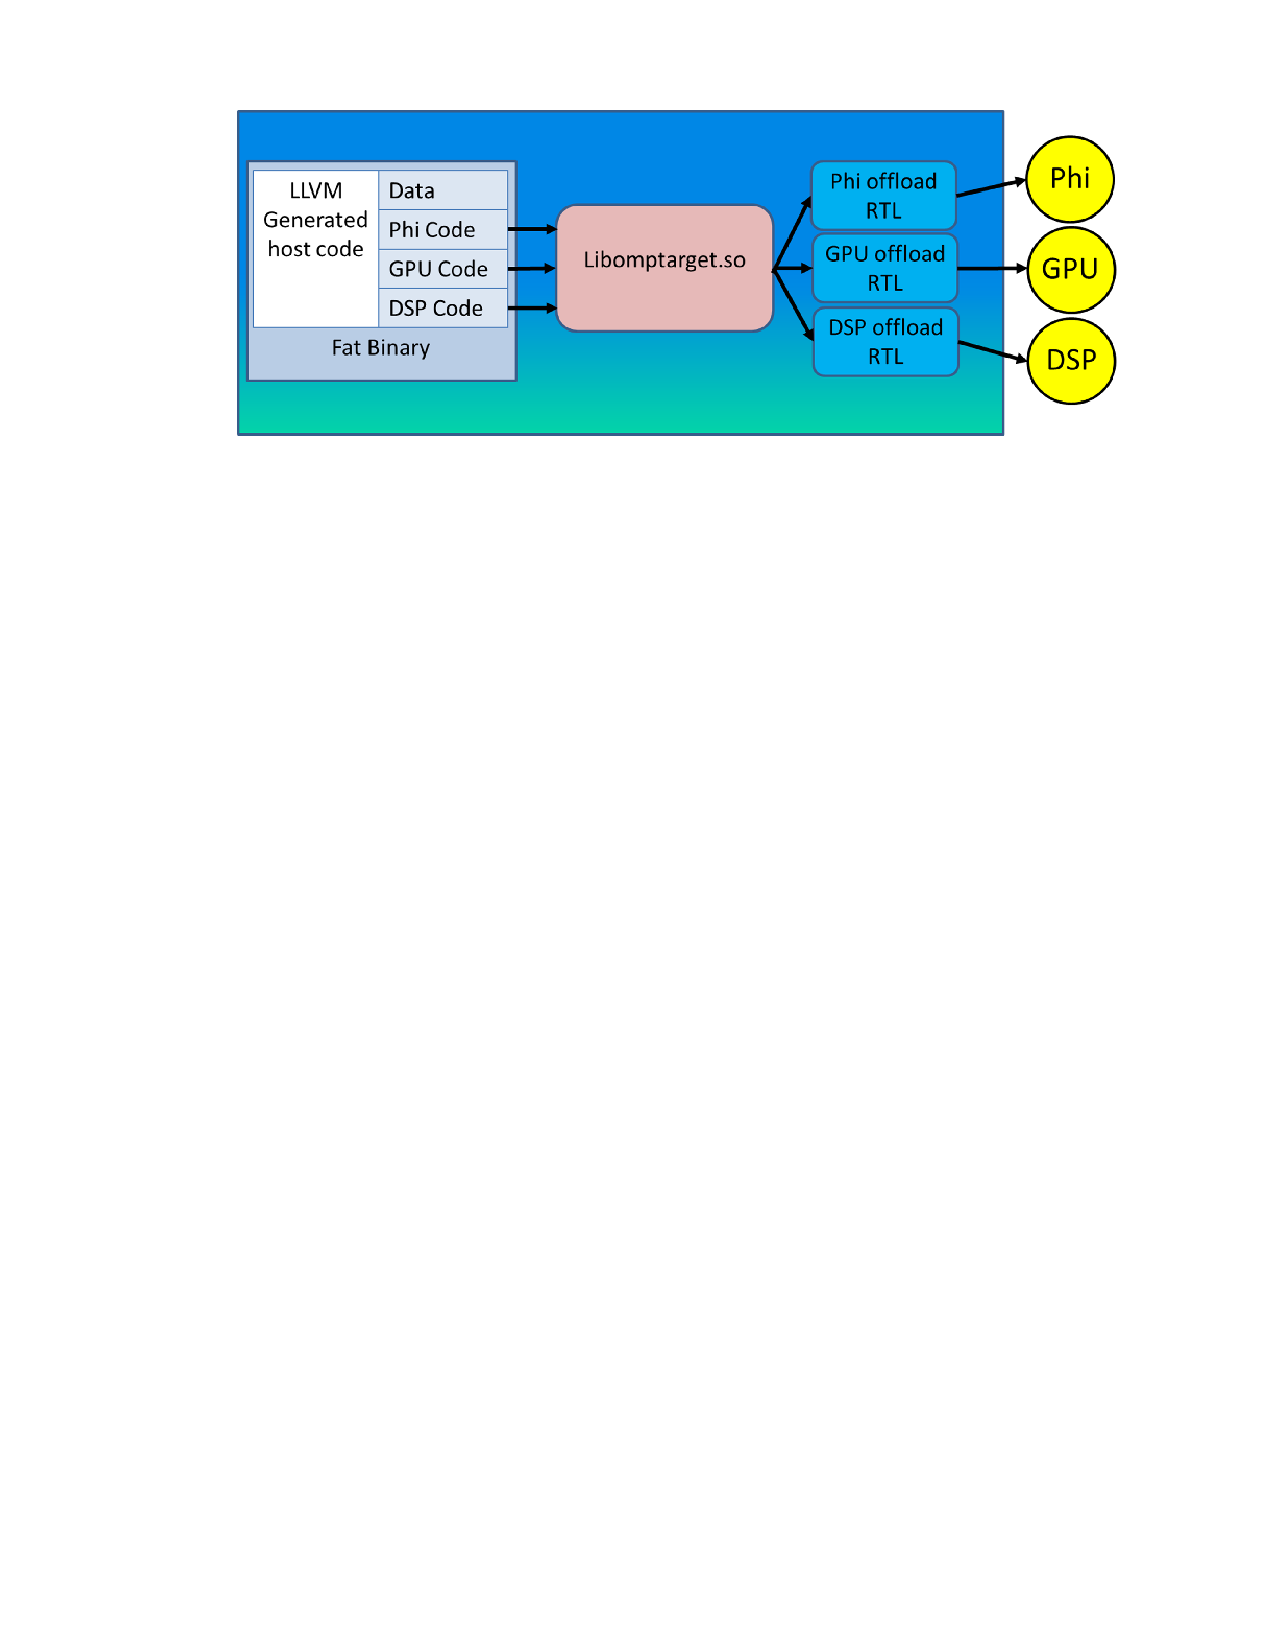
\includegraphics[width=0.9\textwidth]{ImageLibomptarget.pdf}
  \caption{Schematic of \libomptarget{} interface}
  \label{fg:libomptarget_schematic}
\end{figure}

\section{Generation of fat binaries}

To make code generation consistent and straightforward the following scheme is proposed: 
\begin{enumerate}
  \item For each source file provided, the driver spawns the execution of preprocessor, compiler and assembler for the host and each available target device type. This results in the generation of an object file for each target device type. The toolchain of a given target may be modified so that it uses the same definitions (header files) as the host toolchain if that suits the system constraints.

  \item Target linkers combine dedicated target objects into target shared libraries – one for each targetdevice type. The commands passed to the target frontend by the compiler driver always assume the creation of a shared library even if the commands passed to the driver by the user specify otherwise. The driver performs the translation of the host frontend commands to target frontend commands to assure that a target shared library is generated.

  \item The host linker combines host object files into an executable/shared library and incorporateseach target shared libraries as is (no actual linking is done between host and target objects) into its own separate section within the host binary. The format of a binary section for offloading to a specific device is target-dependent and will be thereafter handled by the target RTL at runtime.

  \item A new driver command-line option \command{–omptargets=T1,...,Tn} where \command{Ti} are valid target triples that specify which target device types the user wants to support in the execution of OpenMP target regions. An example, of the invocation of the compiler would be:
  \\ ~ \\
  \command{clang -–fopenmp -–target powerpc64-ibm-linux-gnu\\ –-omptargets=nvptx64-nvidia-cuda,x86-pc-linux-gnu foo.c bar.c –-o foobar.bin}
  \\ ~ \\
  for a hypothetical system where the host is a PowerPC processor and the available target device types are an NVIDIA GPU and x86 processor.

  \item For each source file passed to the driver a unique object file is created for each target device type. The naming convention for a target object file is to append a suffix \command{tgt-<some-target-triple>} to the host object file name. At link time the driver forwards the target object files to the corresponding target toolchain. This mechanism underlies the compiler support for separate compilation. For example:
  \\ ~ \\
  \command{clang –-fopenmp –-target powerpc64-ibm-linux-gnu\\ –-omptargets=nvptx64-nvidia-cuda,x86-pc-linux-gnu foo.c --c}
  \\ ~ \\
  produces the files \command{foo.o}, \command{foo.o.tgt-nvptx64-nvidia-cuda} and \command{foo.o.tgt-x86-pc-linux-gnu}. Then the command:
  \\ ~ \\
  \command{clang –-fopenmp –-target powerpc64-ibm-linux-gnu\\ –-omptargets=nvptx64-nvidia-cuda,x86-pc-linux-gnu foo.o –-o foo.bin}
  \\ ~ \\
  instructs the compiler to locate and forward the files \command{foo.o.tgt-nvptx64-nvidia-cuda} and\command{foo.o.tgt-x86-pc-linux-gnu.o} to the \command{nvptx64-nvidia-cuda} and \command{x86-pc-linux-gnu} toolchains, respectively, so they can be properly linked before being embedded in the host binary.

\end{enumerate}

The resulting host executable/shared library will depend on the offload runtime library -– \libomptarget{}. This library will handle the initialization of target RTLs and translate the offload interface from compiler-generated code to the target RTL during program execution.

\section{The libomptarget.so interface}
The offload library implements the OpenMP 4.0 user-level runtime library routines:
\begin{itemize}
  \item \code{void omp_set_default_device(int device_num)}

  \item \code{int omp_get_default_device(void)}

  \item \code{int omp_get_num_devices(void)}

  \item \code{int omp_is_initial_device(void)}
\end{itemize}

The offload library implements the following compiler-level runtime library routines:
\begin{itemize}

  \item \code{void __tgt_register_lib(__tgt_bin_desc* desc)}\\

    Register the \libomptarget{} library and initialize target state (i.e. global variables and target entry points) for the current host shared library/executable and the corresponding target execution images that have those entry points implemented. This does not trigger any execution in any target as any real work with the target device can be postponed until the first target region is encountered during execution. This function is expected to appear only once per host shared library/executable in the .init section and is called before any constructors or static initializers are called for the host. The name of the caller of \code{__tgt_register_lib} follows the same pattern of the C++ initializers in Clang and is set to \code{_GLOBAL__A_000000_OPENMPTGT}. 

  \item \code{void __tgt_target_data_begin(int32_t device_id, int32_t num_args, void** args_base, void** args, int64_t *args_size, int32_t *args_maptype)}\\

    Initiate a device data environment. It maps variables from the host data environment to the device data environment by recording the mapping between the associated variables’ references used in the host and target into the \libomptarget{} internal structures. The associated variables in the target device data environment are initialized according to the map-type. In the event a given associated variable has already been mapped in other enclosing device data environment, no action is taken for that variable.

  \item \code{void __tgt_target_data_end(int32_t device_id, int32_t num_args, void** args_base, void** args, int64_t *args_size, int32_t *args_maptype)}\\

    Close a device data environment. It removes mapped variables from the current device data environment, releases target memory and destroy the mappings created by the \code{__tgt_target_data_begin()} call that initiated the current device data environment. It assigns host variables the value of the corresponding device data environment variable according to the map-type.

  \item \code{void __tgt_target_data_update(int32_t device_id, int32_t num_args, void** args_base, void** args, int64_t *args_size, int32_t *args_maptype)}\\

    Make the value of a set of variables consistent between the host device and a target device. If avariable’s map type is \mfrom{}, use the value of the variable on the target device. If a variable’s map type is \mto{}, use the value of the variable on the host device.
    
  \item \code{int32_t __tgt_target(int32_t device_id, void *host_addr, int32_t num_args, void** args_base, void** args, int64_t *args_size, int32_t *args_maptype)}\\

    Perform the same actions as \code{__tgt_target_data_begin} in case \code{arg_num} is non-zero and launch the execution of the target region on the target device; if \code{arg_num} is non-zero after the region execution is done it also performs the same action as \code{__tgt_target_data_end} above. If the offloading fails, an error code is returned, which notifies the caller to transfer execution to the appropriate host region. The return code can be used as an error code which will give the compiler and run-time the freedom to implement optimized behaviors.

  \item \code{int32_t __tgt_target_teams(int32_t device_id, void *host_addr, int32_t num_args, void** args_base, void** args, int64_t *args_size, int32_t *args_maptype, int32_t num_teams, int32_t thread_limit)}\\

    This is an extension of \code{__tgt_target} where the caller is able to specify the (maximum) number of teams and threads in each team that \libomptarget{} should start. It reflects the common nesting of the pragma target with the teams one, in OpenMP 4.0. 

\end{itemize}

All the \code{__tgt_target...} calls presented above perform an initial check to understand if the target specified by \code{device_id} was already initialized, and if not, triggers that initialization. The information registered by \code{__tgt_register_lib} is used to accomplish that.

\subsection{Arguments for the libomptarget.so calls}
The following describes the arguments used by the \libomptarget{} interface and how they are used.

\noindent\rule{\textwidth}{0.4pt}

\code{__tgt_bin_desc* desc} points to a constant data struct statically defined by the compiler:
\begin{lstlisting}
struct __tgt_bin_desc{
  uint32_t NumDevices; 
  __tgt_device_image *DeviceImages; 
  __tgt_offload_entry *EntriesBegin;
  __tgt_offload_entry *EntriesEnd; 
};
\end{lstlisting}

\code{NumDevices} is the number of device types whose execution image was generated by the compiler in order to implement some of the offloading entry points. The device types are specified by the user during the invocation of the compiler by passing the flag \command{–omptargets=T1,...,Tn} where \command{Ti} is the triple of a target the user wants to support. NumDevices equals n in this case. 

\code{DeviceImages} is a pointer to an array of NumDevices elements, whose element type is:
\begin{lstlisting}
struct __tgt_device_image{
  void *ImageStart;
  void *ImageEnd;
  __tgt_offload_entry *EntriesBegin;
  __tgt_offload_entry *EntriesEnd; 
};
\end{lstlisting}
%
where ImageStart and ImageEnd contain the addresses where a target image associated to the current host executable/shared library for a given device type starts and ends, respectively. ImageEnd is non-inclusive, i.e. it points to the byte immediately after the target image ends.

\code{EntriesBegin} and \code{EntriesEnd} point to the first and last element of an array that contains the information of each global variable and target entry point that require a map between host and target. These pointers are present in both \code{__tgt_bin_desc} and \code{__tgt_device_image} so that the target dependent runtime (see section 5) can use this information as well to more easily retrieve the entries from the target image (e.g. to retrieve the symbol names of the entries – see below). 

Each element of the array pointed by \code{EntriesBegin} has type:
\begin{lstlisting}
struct __tgt_offload_entry{
  void *addr;
  char *name;
  int64_t size;
  };
\end{lstlisting}
%
where \code{addr} is the address of that global variable or entry point in the host, name is the name of the 
symbol that refers to that global variable or entry point, and size is the size in bytes of the global variable or zero if it is an entry point. If the address field is set to \code{NULL}, the corresponding entry in the table is not supported by the target device associated to this table.

\noindent\rule{\textwidth}{0.4pt}

\libomptarget{} has to be able to map the host entries to the corresponding device entries.

There are different strategies that can be used for mapping the entries. The simplest one is to use the names of the entries for the mapping by performing a name-based search using the name field of the \code{__tgt_offload_entry}. The field name is useful for targets whose runtime requires access to the symbol names in order to locate the correspondent address in the target image. The array that starts at EntriesBegin is built by the compiler in conjunction with the linker, which forwards sequences of entries of different compilation units to the same binary section. In case target and host toolchains can provide strict ordering for both target and host tables – then the mapping can be done by the sequence number of the entry. The frontend ensures that the global variables/entries follow the same order they appear in the source file. Entries associated with static initializers and global destructors are appended to the end of the entries array (i.e. after the global variables themselves and the entries associated with target regions) in the same order they are required in the program. 

\begin{example}
\lstset{basicstyle=\scriptsize,frame=single}
\begin{lstlisting}
#pragma omp declare target
class C{
  C() {// ctor of C}
  ~C() {//dtor of C}
};

C a;
#pragma omp end declare target

foo(){
  #pragma target
  { //target region 1 }
}

#pragma omp declare target
C b;
#pragma omp end declare target

bar(){
  #pragma target
  { //target region 2 }
}
\end{lstlisting}
\lstset{basicstyle=\small\bfseries,frame=none}
\caption{Motivational example for the ordering of entries.}
\label{ex:EntriesOrdering}
\end{example}
%
E.g. in the sample program in Example~\ref{ex:EntriesOrdering}, the order of the entries will be: global variable \code{a}, target region 1, global variable \code{b}, target region 2, caller of the constructor of \code{a} and \code{b} (\code{a} and \code{b} have the same priority), caller of the destructors of \code{a} and \code{b}. The callers of the constructors and destructors are always launched with a single thread and team. If the toolchain of a given target does not preserve the order, that target runtime may consult the host entries and obtain the same order of the symbols based on the name.

\noindent\rule{\textwidth}{0.4pt}

\code{int32_t device_id} is an integer that uniquely identifies a given target. In the first call of \code{__tgt_register_lib}, \libomptarget{} detects the available target dependent RTLs in the system and uses them to query the number of devices of each type that are ready to be used. If $A$ devices of type \command{T1} and $B$ devices of type \command{T2} are found, where \command{T1} and \command{T2} are the types specified by the user with \command{-–omptargets=T1,T2}, \code{device_id} $[0,A[$ will map to devices of type \command{T1} and \code{device_id} $[A,A+B[$ will map to devices of type \command{T2}. If \code{device_id} is greater or equal than $A+B$, the call where it is used will fail and no action will be taken by \libomptarget{}. On top of the positive values used for \code{device_id}, the compiler also employs three reserved values:

\begin{itemize}
  \item \code{device_id = -1}: informs the runtime that the user has not specified any device ID, and therefore the default must be used, which may be specified through an environment variables as specified in the OpenMP 4.0 specification.

  \item \code{device_id = -2}: informs the runtime that the target action must be performed on all available devices and can be delayed until the first time the device action is invoked with a device ID greater or equal to \code{-1}. This is mainly used to call C++ global initializers, which only need to be called if the device is eventually used for executing at least one target region.

  \item \code{device_id = -3}: informs the runtime that the target action must be performed on all available devices that were ever used in the current library. This is mainly used to call C++ destructors, which are only required if that device was used before.
\end{itemize}

\noindent\rule{\textwidth}{0.4pt}

\code{int32_t num_args} is the number of data pointers that require a mapping.

\noindent\rule{\textwidth}{0.4pt}

\code{void** args} is a pointer to an array with \code{num_args} arguments whose elements point to the first byte of the array section that needs to be mapped.

\noindent\rule{\textwidth}{0.4pt}

\code{int64_t* args_size} is a pointer to an array with \code{num_args} arguments whose elements contain the size in bytes of the array section to be mapped.

\noindent\rule{\textwidth}{0.4pt}

\code{void** args_base} is a pointer to an array with \code{num_args} arguments whose elements point to the base address of the declaration the mapping refers to. \code{args_base} differs from args if an array section does not start at zero. \libomptarget{} needs to know the base addresses in order to relate mapped data with target region arguments that are dereferenced in the target region body.

\noindent\rule{\textwidth}{0.4pt}

\code{int32_t *args_maptype} is a pointer to an array with \code{num_args} arguments whose elements contain the required map attributes as specified in the enum:
\begin{lstlisting}
enum tgt_map_type {
  OMP_TGT_MAPTYPE_TO = 0x0001,
  OMP_TGT_MAPTYPE_FROM = 0x0002,
  OMP_TGT_MAPTYPE_ALWAYS = 0x0004,
  OMP_TGT_MAPTYPE_DELETE = 0x0008,
  OMP_TGT_MAPTYPE_MAP_PTR = 0x0010,
  OMP_TGT_MAPTYPE_FIRST_MAP = 0x0020,
  OMP_TGT_MAPTYPE_RETURN_PTR = 0x0040,
  OMP_TGT_MAPTYPE_PRIVATE_PTR = 0x0080,
  OMP_TGT_MAPTYPE_PRIVATE_VAL = 0x0100
};
\end{lstlisting}

\sloppy
\code{OMP_TGT_MAPTYPE_TO} instructs the runtime to copy  host data to the device in a target data begin, target update, or when initiating a target construct.  \code{OMP_TGT_MAPTYPE_FROM} instructs the runtime to copy  device data to the host in a target data end, and target update, or when completing a target construct.  \code{OMP_TGT_MAPTYPE_ALWAYS} forces the copying regardless of the reference count associated with the map.  \code{OMP_TGT_MAPTYPE_DELETE}  forces the unmapping of the object in a target data end or when completing a target construct. \code{OMP_TGT_MAPTYPE_MAP_PTR} forces the runtime to map the pointer variable as well as the pointee variable. This attribute also instructs the runtime to initialize the value of the pointer on the device with the base device address of the pointee mapped variable. 

\code{OMP_TGT_MAPTYPE_FIRST_MAP} instructs the runtime that it is the first occurrence of this mapped variable within this construct.  When used with  the \code{OMP_TGT_MAPTYPE_MAP_PTR}, it instructs the runtime that it is the first occurrence of the pointer mapped variable; a pointee mapped variable is considered by definition as its first occurrence. This attributes is used to determine when to update the reference count associated with a mapped variable needs, and when to include the base device address of a mapped variables in the target var argument. 

\code{OMP_TGT_MAPTYPE_RETURN_PTR} instructs the runtime to returns the base device address of the mapped variable in the corresponding \code{base_args} entry. When used with  the \code{OMP_TGT_MAPTYPE_MAP_PTR} attribute, the runtime returns the base device address of the pointer mapped variable. This attribute is used to implement the \code{use_device_ptr} clause.

The next two flags indicate to the runtime that it is not dealing with mapped variables.  First, \code{OMP_TGT_MAPTYPE_PRIVATE_PTR} informs the runtime that the described variable is a private variable. First-private variables are indicated by using the  \code{OMP_TGT_MAPTYPE_TO}  attribute in conjunction with the private attribute. The runtime is responsible for allocating the device memory associated with the variable, but it is not mapped as it is private. Second, \code{OMP_TGT_MAPTYPE_PRIVATE_VAL} instructs the runtime to simply forward the value of the \code{args_base} parameter to the target construct.  This attribute is used to implement the \code{is_device_ptr} clause. This attribute can also be used by the compiler to forward small first-private values directly to the device via the target var argument. No allocation of memory occurs with this attribute.

The fields in the interface are used in three different ways depending on the presence of the \code{OMP_TGT_MAPTYPE_MAP_PTR} and \code{OMP_TGT_MAPTYPE_PRIVATE_VAL} attributes.

%
\begin{itemize}
  \item Variables without the \code{OMP_TGT_MAPTYPE_MAP_PTR} and \code{OMP_TGT_MAPTYPE_PRIVATE_VAL} attributes.  \code{args_base} contain the references to the variables that are being mapped.  \code{args} points to the beginning of the data as requested by the user. For scalars, \code{args_base}  and \code{args} are identical. For arrays, the user may request a subset of arrays, in which case \code{args} points to the beginning of these array subsets. Similarly, for struct, the user may request to map only a subset of the struct fields, in which case  \code{args} points to the first fields of these structs. \code{args_size} contains the sizes of the variables, or the appropriate subsets of the variables, that are being mapped. \code{args_maptype} contains the attributes that control the data movement between host and device.

  \item Variables with the \code{OMP_TGT_MAPTYPE_MAP_PTR} attribute and without the \code{OMP_TGT_MAPTYPE_PRIVATE_VAL} attribute. Arguments for mapped pointers describe both the pointer and pointee variables.  \code{args_base} contains the references to the pointer variables to be mapped.  If needed, the references to the pointee variables are found by dereferencing the \code{args_base} pointers. \code{args} contains the beginning of the data of the pointee variables.   For arrays and structs, \code{args} points to the beginnings of the subsets of the pointee variables that are being mapped. \code{args_size} contains the sizes of the pointee variables, or the appropriate subset of the variables, that are being mapped. \code{args_maptype}  contains the attributes that control the data movement of the pointee variable between host and device. By definition, the values of the mapped pointer variables on the device are never copied back to the host.
  
  \item Variables with the \code{OMP_TGT_MAPTYPE_PRIVATE_VAL} attribute. The values to forward are found in the \code{args_base} arguments;  \code{args} and \code{args_size} values are unused.
%
\end{itemize}

\fussy

Zero-length array references are identified by their \code{args_size} values of zero; and since they cannot have an offset, their \code{args} values are unused.

Table~\ref{tb:PointersMapping} shows the content of the arrays passed to \code{__tgt_target_data_begin()} and \code{__tgt_target} as result of the \dtargetdata{} and \dtarget{} pragmas in Example~\ref{ex:PointersMapping}.

Variable \code{i} is also passed to \code{__tgt_target} because it is captured in the body of the target region and are therefore arguments to the target region. Variable \code{pA} is also captured, and as captured pointers, it is mapped as a zero-length array. The \libomptarget{} implementation will detect that \code{s1} was mapped before and will not take any action to map this variables again. Variable \code{C} illustrates the use of \code{use_device_ptr} and \code{is_device_ptr}.

The arguments that are used to invoke the target kernel (see void \code{*target_vars_ptr} in Section~\ref{sc:TargetRTLInterface}) consist of the mapped base address of all elements. In the example above the arguments would be \code{&di, &dpA, &dA[0], &ds1, &dC}, where \code{dX} is the map of {X} in the device.

\begin{example}
\lstset{basicstyle=\scriptsize,frame=single}
\begin{lstlisting}
// N, M and S are constants
foo(){
  int A[N], D[N], *pA, i;
  struct S1 {int x, y, B[M], *pB, u, v; } s1;
  int C[N];
  
  pA = (int*)malloc(N*sizeof(int)); 
  s1.pb = (int*)malloc(M*sizeof(int)); 

  #pragma omp target data map(pA[0:M], s1, C) use_device_ptr(C)
  { 
    /* C now correspond to the device pointer associated with mapped variable C, and can be used in a Cuda call, for example */
    #pragma omp target map(to: A[S:M], s1.B[0:M]) map(from:s1.pb[0:M]) is_device_ptr(C) firstPrivate(D[0:M])
    {
      for (i=S; i<M; ++i){ 
        ++A[i]; 
        --pA[i]; 
        s1.pb[i-S] = s1.B[i-S] + A[i]*pA[i] - C[i] * D[i]; 
      }
    }
  }
}
\end{lstlisting}
\lstset{basicstyle=\small\bfseries,frame=none}
\caption{Example requiring mapping of pointer.}
\label{ex:PointersMapping}
\end{example}

\begin{table}
\centering
\begin{tabular}{c|c|c|p{3cm}|p{3.5cm}}
%
\code{args_base} & 
\code{args} & 
\code{args_size} & 
\code{args_maptype} &
comment \\\hline
%
\multicolumn{4}{c}{\cellcolor{gray!20}\code{\#pragma omp target data - __tgt_target_data_begin()}} \\\hline
%    map(pA[S:M])
\code{pA} & 
\code{&pA[0]} & 
\code{M*sizeof(int)} & 
\code{TO | FROM | FIRST_MAP} &
mapped array subset\\\hline
%  map(s1)
\code{&s1} & 
\code{&s1} & 
\code{sizeof(S1)} & 
\code{TO | FROM | FIRST_MAP} &
mapped struct\\\hline
%  map(C) use_device_ptr(C)
\code{&C} & 
\code{&C} & 
\code{N*sizeof(int)} & 
\code{TO | FROM | FIRST_MAP | RETURN_PTR} &
mapped array for which the compiler want the device address\\\hline
%
\multicolumn{4}{c}{\cellcolor{gray!20}\code{\#pragma omp target - __tgt_target()}} \\\hline
%  map(to: pA[0:0])
\code{pA} & 
\code{undefined} & 
\code{0} & 
\code{TO | FIRST_MAP} &
zero-length first-private pointer to a mapped array\\\hline
% map(to: A[S:M])
\code{&A} &
\code{&A[S]} &
\code{sizeof(int)} & 
\code{TO | FIRST_MAP} &
mapped array\\\hline
% map(to s1.B[0:M] ... s1.pb)
\code{&s1} & 
\code{&s1.B[0]} & 
\code{M*sizeof(int)+sizeof(void *)} & 
\code{FIRST_MAP} &
allocation of mapped struct subset\\\hline 
% map(to s1.B[0:M])
\code{&s1} & 
\code{&s1.B[0]} & 
\code{M*sizeof(int)} & 
\code{TO} &
memory move for subset of mapped struct\\\hline 
% map(from s1.pB[0:M])
\code{&s1.pB} & 
\code{&s1.pB[0]} & 
\code{M*sizeof(int)} & 
\code{FROM | MAP_PTR} &
mapped pointer and pointee array subset\\\hline 
% is_device_ptr(C)
\code{&C} & 
\code{undefined} & 
\code{undefined} & 
\code{PRIVATE_VAL} &
mapped pointer and pointee array subset\\\hline 
%  firstprivate(i) 
\code{i} & 
\code{undefined} & 
\code{undefined} & 
\code{PRIVATE_VAL} &
first-private scalar passed as value\\\hline%  firstprivate(D) 
\code{&D} & 
\code{&D[0]} & 
\code{M*sizeof(int)} & 
\code{PRIVATE_PTR  | TO} &
first-private array\\\hline
%
\end{tabular}
\caption{Contents of the arrays passed through the interface for Example~\ref{ex:PointersMapping}. \code{OMP_TGT_MAPTYPE_} prefixes are omitted for conciseness. }
\label{tb:PointersMapping}
\end{table}















\section{Target RTL synchronous interface}\label{sc:TargetRTLInterface}

As it can be derived from the previous Sections, a target RTL must provide the following capabilities:

\begin{itemize}
  \item \code{int32_t __tgt_rtl_number_of_devices()} – return the number of available devices of the type supported by the target RTL.

  \item \code{int32_t __tgt_init_device(int32_t device_id)} – initialize the specified device. In case of success return 0; otherwise return an error code. 

  \item \code{tgt_target_table* __tgt_rtl_load_binary(int32_t device_id, __tgt_device_image *image)} – pass an executable image section described by image to the specified device and prepare an address table of target entities. In case of error, return \code{NULL}. Otherwise, return a pointer to the built address table. Individual entries in the table may also be \code{NULL}, when the corresponding offload region is not supported on the target device (see previous Section).
  
  \item \code{int32_t __tgt_rtl_is_valid_binary(__tgt_device_image *image)} - return an integer different from zero if the provided device image can be supported by the runtime. The functionality is similar to comparing the result of \code{__tgt_rtl_load_binary} to null. However, this is meant to be a lightweight query to determine if the RTL is suitable for an image without having to load the library, which can be expensive.

  \item \code{void* __tgt_rtl_data_alloc(int32_t device_id, int64_t size)} – allocate data on the particular target device, of the specified size. Return address of the allocated data on the target that will be used by \libomptarget{}to initialize the target data mapping structures. These addresses are used to generate a table of target variables to pass to \code{__tgt_rtl_run_region()}. The \code{__tgt_rtl_data_alloc()}returns \code{NULL} in case an error occurred on the target device.

  \item \code{int32_t __tgt_rtl_data_submit(int32_t device_id, void *target_ptr, void *host_ptr, int64_t size)} – pass the data content to the target device using the target address. In case of success, return zero. Otherwise, return an error code.

  \item \code{int32_t __tgt_rtl_data_retrieve(int32_t device_id, void *host_ptr, void *target_ptr, int64_t size)} – retrieve the data content from the target device using its address. In case of success, return zero. Otherwise, return an error code.

  \item \code{int32_t __tgt_rtl_data_delete(int32_t device_id, void *target_ptr)} – de-allocate the data referenced by \code{target_ptr} on the device. In case of success, return zero. Otherwise, return an error code.

  \item \code{int32_t __tgt_rtl_run_target_region(int32_t device_id, void *target_entry_ptr, void **target_vars_ptr, int32_t arg_num)} – transfer control to the offloaded entry on the target device; \code{target_vars_ptr} is a table to store the target addresses of all variables used in the target entry code. Entries in \code{target_vars_ptr} match the order of the variables passed in the \code{arg_host_ptr} argument passed to the target region. In case of success, return zero. Otherwise, return an error code.

  \item \code{int32_t __tgt_rtl_run_target_team_region(int32_t device_id, void *target_entry_ptr, void **target_vars_ptr, int32_t arg_num, int32_t num_teams, int32_t thread_limit)} – transfer control to the offloaded entry on the target device; \code{target_vars_ptr} is a table to store the target addresses of all variables used in the target team entry code. Entries in \code{target_vars_ptr} match the order of the variables passed in the \code{arg_host_ptr} argument passed to the target team region. In case of success, return zero. Otherwise, return an error code.

\end{itemize}

For each platform there can be a dedicated set of error numbers defined \libomptarget{} assumes that zero is returned in case of success, independently of the target device. If a given system supports shared memory, the target RTL implementation of the \code{__tgt_rtl_data_*()} can optionally not take any action, as host and target device can operate on the same data.


%%%%%%%%%%%%%%%%%%%%%%%%%%%%%%%%%%%%%%%%%%%%
%%%%%%%%%%%%%%%%%%%%%%%%%%%%%%%%%%%%%%%%%%%%

\section{Target RTL asynchronous interface} \label{sc:TargetRTLInterfaceAsync}

The asynchronous RTL interface augment the calls seen in Section~\ref{sc:LibomptargetAsync} and Section~\ref{sc:TargetRTLInterface}. First, it implements the RTL-specific calls related to offloading dependences.

\begin{itemize}
  \item \code{void __tgt_rtl_init_dep(tgt_callback_fct completion_callback)} 
  \item \code{int32_t __tgt_rtl_enforce_dep(int32_t from_device_id, int32_t to_device_id, tgt_event_t completion_event)} 
  \item \code{void __tgt_rtl_release_dep(tgt_sync_event_t completion_event)} 
  \item \code{int32_t __tgt_rtl_process_dep()} 
 \end{itemize}

Second, the asynchronous RTL interface provides the following asynchronous data transfer and offloading calls. 

\begin{itemize}
  \item \code{int32_t __tgt_rtl_async_dep(int32_t device_id, int32_t num_dep_events, tgt_event_t *dep_events, tgt_event_t *completion_event)} 
  \item \code{int32_t __tgt_rtl_async_data_submit(int32_t device_id, void *target_ptr, void *host_ptr, int64_t size, int32_t num_dep_events, tgt_event_t *dep_events, tgt_event_t *completion_event)} 
  \item \code{int32_t __tgt_rtl_async_data_retrieve(int32_t device_id, void *host_ptr, void *target_ptr, int64_t size, int32_t num_dep_events, tgt_event_t *dep_events, tgt_event_t *completion_event)} 
  \item \code{int32_t __tgt_rtl_async_run_target_region(int32_t device_id, void *target_entry_ptr, void **target_vars_ptr, int32_t arg_num, int32_t num_dep_events, tgt_event_t *dep_events, tgt_event_t *completion_event)} 
  \item \code{int32_t __tgt_rtl_async_run_target_team_region(int32_t device_id, void *target_entry_ptr, void **target_vars_ptr, int32_t arg_num, int32_t num_teams, int32_t thread_limit, int32_t num_dep_events, tgt_event_t *dep_events, tgt_event_t *completion_event)} 
  \end{itemize}
  
 In the above list, the first call requires no computation or communication, it just enables \libomptarget{} to summarize all of the synchronization events (listed in \code{dep_event}) into a single event, \code{completion_event}, which must occur after all listed events are completed. Note that the \code{dep_events} synchronization event may now also include dependences on the completion of data transfers initiated by \libomptarget{}. For devices that support the concept of streams, it is expected that the new operation will be queue up in the stream associated with the first synchronization event in \code{dep_event}.
  

\end{document}